\begin{figure}
	\centering
	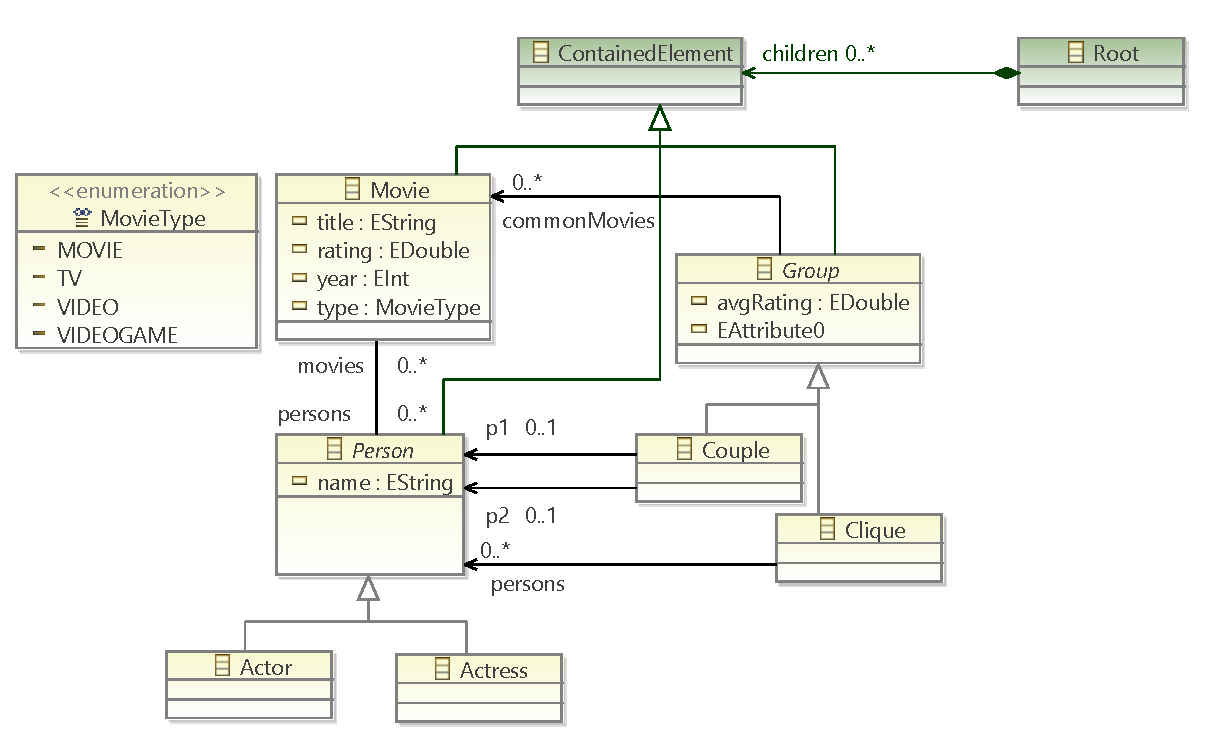
\includegraphics[width=.7\textwidth]{metamodel.pdf}
	\caption{Our extended metamodel.}\label{fig:metamodel}
\end{figure}

\section{Solution}
\label{sec:solution}

\subsection{Specification}

In the provided Ecore model, no containment hierarchy is used and all objects are held in the \textsf{contents} list of the EMF resource. However, this also means that the performance of the transformation can be affected by the resource implementation used (since it will determine the implementation of the list operations).

For performance considerations, we used an extended version of the metamodel, which has a \textsf{Root} object (see \figref{fig:metamodel}). This object serves as a container for all \textsf{Group}, \textsf{Movie} and \textsf{Person} objects. According to our experiments, this increases the speed of the pattern matching by a factor of two.

We ensured that our solution works with the models provided and also persists outputs in a format that does not include the root element. This way, the transformation part of our solution is independent of resource implementation (binary, UUID-based, regular XMI, etc.).

\subsection{Patterns and Transformations}

\subsubsection{Task 1: Generating Test Data}
\label{t1}

The synthetic test data is generated in Xtend (see Listing~\ref{app:xtend:task1}). The code tightly follows the specification defined in the case description~\cite{Horn14}.
Since the task is simple model construction without any querying, \incquery{} is not used in this task. 

\subsubsection{Task 2: Finding Couples}
\label{t2}

Couples are listed with the following pattern:

\listingIQPL{./src/couple.eiq}

Note that the \textsf{cast} pattern returns the names of persons that play in a given movie. This is important since the names of the persons can be used to avoid symmetric matches in the \textsf{personsToCouple} pattern by sorting.
The \textsf{Couple} objects are created and configured in Xtend (see \textsf{createCouples} in line~\ref{xform:createCouples} of Listing~\ref{app:xtend:xform}). This includes setting the \textsf{p1} and \textsf{p2} references using a \textsf{personName} pattern and computing the \textsf{commonMovies} by simple set intersection operators (\textsf{retainAll}).

\subsubsection{Task 3: Computing Average Rankings}
\label{t3}

The average rankings are computed in Xtend by calculating the mean of the \textsf{rating} attributes of a couple's common movies (see \textsf{calculateAvgRatings} in line~\ref{xform:calculateAvgRatings} of Listing~\ref{app:xtend:xform}). The movies are enumerated with the following pattern:

\listingIQPL{./src/commonMoviesOfCouple.eiq}

\subsubsection{Extension Task 1: Compute Top-15 Couples}
\label{et1}

This task is mostly implemented in Xtend (see \textsf{topGroupByRating} in line~\ref{xform:topGroupByRating} and \textsf{topGroupByCommonMovies} in line~\ref{xform:topGroupByCommonMovies} of Listing~\ref{app:xtend:xform}), however, it uses the \textsf{groupSize} pattern in order to filter the groups with the particular number of members.

\listingIQPL{./src/groupSize.eiq}

This pattern uses the \textsf{count find} construct which computes the number of matches for a given pattern. 
Additionally, specific comparators are used to sort and determine the top-15 lists by rating or number of common movies (see Listing~\ref{app:xtend:comparator}). 

\subsubsection{Extension Task 2: Finding Cliques}
\label{et2}

The pattern for finding cliques is implemented similarly to the \textsf{personsToCouple} pattern~\ref{t2}. The pattern for 3-cliques is defined as follows:

\listingIQPL{./src/clique-3.eiq}

The creation of cliques is done similarly to couples (see \textsf{createCliques} in line~\ref{xform:createCliques} of Listing~\ref{app:xtend:xform}). However, this pattern has a redundant check constraint, as $P_1 < P_2$ and $P_2 < P_3$ already imply $P_1 < P_3$. This works as a hint for the query engine and allows it to filter the permutation of the results (e.g.\ $(a_2, a_1, a_3), (a_1, a_3, a_2), \ldots)$) earlier.

To achieve high query performance, patterns for 4- and 5-cliques are defined manually. For larger cliques ($n > 5$), patterns could be automatically generated using code generation techniques.

\paragraph{General solution for $n$-cliques.} We also provide the outline for a more general solution (for arbitrary $n$ values). For the sake of clarity, we will refer to couples as 2-cliques. In this approach, the cliques are built iteratively. Suppose we already have all $k$-cliques in the graph (e.g.\ we already added the 2-, 3-, 4- and 5-cliques with the previous patterns). To get the $(k+1)$-cliques, we look for a group $g_0$ and a person $p_0$ that (i) have at least 3 movies in common, (ii) $ g = g_0 \cup \left\{p_0\right\} $ is a group that is not a subset of any other groups (see Figure~\ref{fig:positive-pattern}).

Formally, (ii) can be expressed as $ \left(\not\exists g'\right): g \subseteq g' $. Using $ g = g_0 \cup \left\{p_0\right\} $, we derive the following expression $\left(\not\exists g'\right): \left(g_0 \subseteq g'\right) \wedge \left(p \in g'\right)$. The $g_0 \subseteq g'$ expression can be formulated as follows: $\left(\forall p_0 \in g_0\right): p_0 \in g'$. As the \iqpl{} does not have a universal quantifier, we rewrite this using the existential quantifier: $\left(\not\exists p_0 \in g_0\right): p_0 \not\in g'$.

\begin{figure}
	\centering
	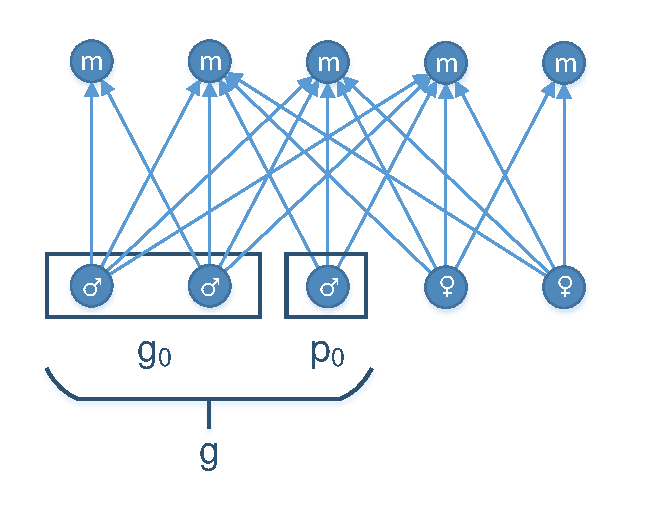
\includegraphics[width=.5\textwidth]{positive-pattern.pdf}
	\caption{Matching 3-clique groups in the positive test pattern. $g_0$ is a couple.}\label{fig:positive-pattern}
\end{figure}

The resulting expression for condition (ii) is the following: $\left(\not\exists g'\right): \left(\left(\not\exists p_0 \in g_0\right): p_0 \not\in g'\right) \wedge \left(p \in g'\right)$. This is equivalent to the following \incquery{} pattern:

\listingIQPL{./src/subset.eiq}

Based on the \textsf{subsetOfGroup} pattern, we may implement the \textsf{nextClique} pattern like follows:

\listingIQPL{./src/clique.eiq}

Given a model containing all $k$-cliques, the \textsf{nextClique} pattern is capable of determining the $(k+1)$-cliques. While this solution is functionally correct, it only works for very small input models and hence is omitted from our implementation.

\subsubsection{Extension Task 3: Compute Average Rankings for Cliques}
\label{et3}

The average rankings are computed the same way as in \emph{task 3} (section~\ref{t3}).

\subsubsection{Extension Task 4: Compute Top-15 Cliques}
\label{et4}

The top 15 average rankings are computed the same way as in \emph{extension task 2} (section~\ref{et2}).

\subsection{Optimizations}

To increase the performance of the transformations, we used some optimizations.

\begin{itemize}
  \item After the matcher engine produced the initial result set, the engine is turned off. This way, we spare the cost of incrementally maintaining the result set. As the transformation is non-incremental, this does not affect the result of the performance. 
  \item The common movies of the two \textsf{Person} objects are computed from Xtend instead of \incquery{}.
  \item The patterns for 3-, 4- and 5-cliques are implemented manually.
\end{itemize}
 
We looked for \emph{common subpatterns} and extracted them into separate patterns. This results in better performance as the engine can reuse the pattern for each occurrence, and makes the query definition file easier to maintain. For an example, see the \textsf{cast} pattern in~\ref{app:pattern}.

\subsection{Build Automation}

Our solution was developed in the Eclipse IDE. While it is fully functional in Eclipse, it can also be compiled with the Apache Maven~\cite{Maven} build automation tool. This offers a number of benefits, including easy portability and the possibility of continuous integration. The build process uses the Tycho Maven plug-in~\cite{tycho} to build the Eclipse plug-ins defined in the project.

\subsection{Benchmark Results}

The implementation was benchmarked in the SHARE cloud, on an Ubuntu 12.04 64-bit operating system running in a VirtualBox environment. The virtual machine used one core of an Intel Xeon E5-2650 CPU and had 6 GB of RAM.

The benchmark used Maven to build the binary files. The transformations were ran in a timeout window of 10 minutes.

\subsection{Synthetic model}

Results are displayed in \figref{fig:benchmark-results}. The diagram shows the transformation times for creating couples and cliques for synthetic models. The results show that the transformations run in near linear time.

The dominating factor of the running time is the initialization of the query engine. However, after initialization, creating groups can be carried out efficiently.

Furthermore, our experiments showed that the limiting factor for our solution is the memory consumption of the incremental query engine. Given more memory, the solution is capable of transforming larger models as well.

\begin{figure}
	\centering
	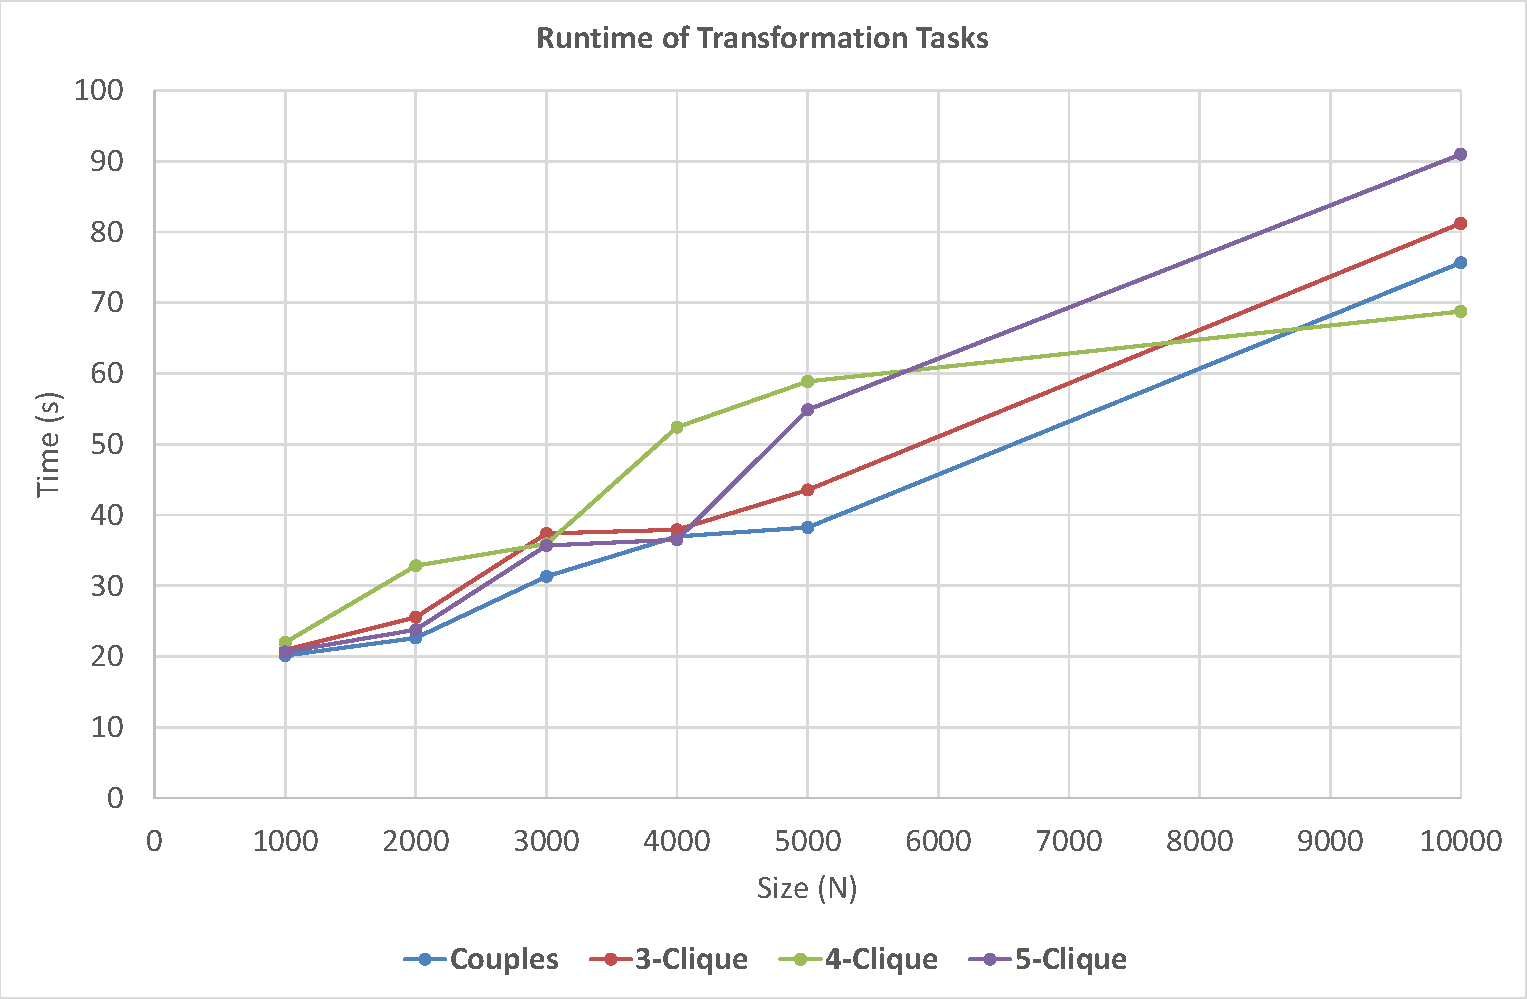
\includegraphics[width=.9\textwidth]{results-full.pdf}
	\caption{Benchmark results.}\label{fig:benchmark-results}
\end{figure}

\subsection{IMDb model}

In the given time range and memory constraints, the transformation of the IMDb model could only generate the couples and 3-cliques for the smallest instance model. Finding the couples took 3 minutes, while finding 3-cliques took 6. However, in case of a live and evolving model, our solution is capable of incrementally running the transformation which in practice results in near instantaneous response time.

\subsection{Transformation Correctness and Reproducibility}

The transformation runs correctly for the provided test cases on SHARE\footnote{\url{http://is.ieis.tue.nl/staff/pvgorp/share/?page=ConfigureNewSession&vdi=Ubuntu12LTS_TTC14_64bit_TTC14-EIQ-imdb.vdi}}, and the source code is also available in a Git repository\footnote{Homepage: \url{https://git.inf.mit.bme.hu/w?p=projects/viatra/ttc14-eiq.git} (use the \texttt{anonymous} user with no password), clone URI: \texttt{https://anonymous@git.inf.mit.bme.hu/r/projects/viatra/ttc14-eiq.git}}. The results of the transformations were spot-checked for both synthetic and IMDb models.  

\subsection{Tool Support for Debugging and Refactoring}

As the transformation is written in two languages, debugging and refactoring is dependent on the tooling for these languages and the capabilities of the query engine. 

Xtend and the \incquery{} pattern editors are based on Xtext, and while provide some refactoring operations. Declarative \incquery{} graph patterns cannot be efficiently debugged at runtime. However, smaller instance models can be loaded into the \emph{Query Explorer} view, which is very handy to the debug matches of the patterns. The engine controller code can be debugged and refactored as well, as it is implemented in Java. Debug messages of the execution engine can be turned on, which prints useful messages about rule firings and activations. Firings of the transformation operations can be debugged by placing breakpoints in the Xtend code.

